\textbf{A.5.1--4. Inputs and frequencies.} The length is $L=25.5(0.0254)=0.6477\ \mathrm{m}$, the initial displacement is $u_{\max}=1.25\ \mathrm{mm}$, and the number of modes is $N=10$. For G3, I use the equal-tempered frequency $f_1=196.0\ \mathrm{Hz}$. Therefore,
\[
\tau_1=\frac1{f_1}=5.102\ \mathrm{ms},\qquad
c=2Lf_1=253.9\ \mathrm{m/s},\qquad
t_{\max}=3\tau_1=15.31\ \mathrm{ms}.
\]
The mode wavenumbers and angular frequencies are $\gamma_j=j\pi/L=(4.850j)\ \mathrm{rad/m}$ and $\omega_j=2\pi f_1j=(1232j)\ \mathrm{rad/s}$ for $j=1,\ldots,10$. The corresponding shapes $U_j(x)=\sin(\gamma_jx)$ are plotted below.

\textbf{A.5.5--6. Modal expansion.} The initial shape is $u_0(x)=u_{\max}x/d$ on $0\le x\le d$ and $u_0(x)=u_{\max}(L-x)/(L-d)$ on $d<x\le L$. Releasing the string from rest sets the initial velocity coefficients to zero. Using the sine modes and their squared norm $L/2$, numerical trapezoidal integration on 2001 points gives
\[
A_j=\frac{2}{L}\int_0^L u_0(x)\sin(\gamma_jx)\,dx,\qquad
u(x,t)=\sum_{j=1}^{10}A_j\sin(\gamma_jx)\cos(\omega_jt).
\]
The three physical pluck positions are $d=323.85$, $161.925$, and $453.39\,\mathrm{mm}$, respectively. The results agree with the closed form $A_j=2u_{\max}\sin(j\pi d/L)/[\pi^2j^2(d/L)(1-d/L)]$ to within $2.8\times10^{-7}\ \mathrm{mm}$. The course notes give the same initial shape and modal expansion in Eqs. (85), (95), (97), and (100), PDF pages 160--162.

\begin{center}\small
\begin{tabular}{rrrr}
\toprule
$j$ & $A_j$ at $d=L/2$ (mm) & $A_j$ at $d=L/4$ (mm) & $A_j$ at $d=0.7L$ (mm)\\
\midrule
1&1.013&0.955&0.976\\
2&0&0.338&-0.287\\
3&-0.113&0.106&0.0414\\
4&0&0&0.0443\\
5&0.0405&-0.0382&-0.0483\\
6&0&-0.0375&0.0197\\
7&-0.0207&-0.0195&0.00761\\
8&0&0&-0.0179\\
9&0.0125&0.0118&0.0121\\
10&0&0.0135&0\\
\bottomrule
\end{tabular}
\end{center}
The graphs show all ten modes, each initial shape and its ten-mode reconstruction, and $u(d,t)$ through three fundamental periods. The bars show the participation factors.
\begin{figure}[H]\centering
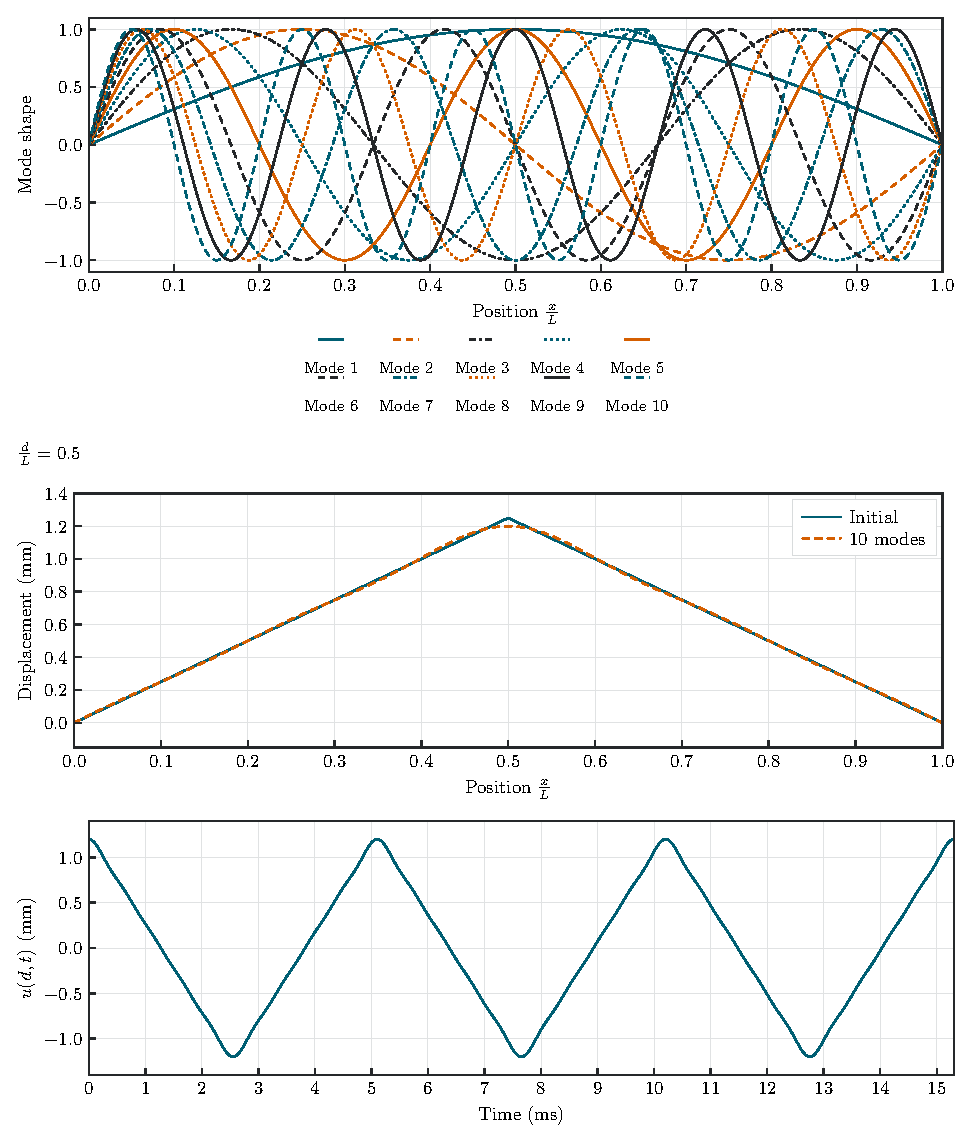
\includegraphics[page=1,width=0.95\linewidth]{figures/generated/solutions/A5.pdf}
\caption{A.5. Ten string modes and the initial shape and response for $d=L/2$.}
\end{figure}
\begin{figure}[H]\centering
\includegraphics[page=2,width=0.95\linewidth]{figures/generated/solutions/A5.pdf}
\caption{A.5. Initial shapes, reconstructions and responses for the remaining pluck locations.}
\end{figure}
\begin{figure}[H]\centering
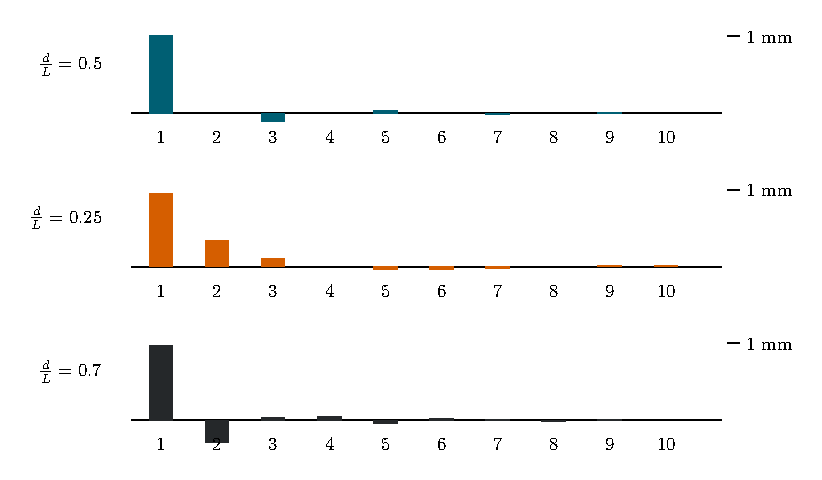
\includegraphics[width=0.8\linewidth]{figures/generated/solutions/A5bars.pdf}
\caption{A.5. Modal participation factors in millimetres.}
\end{figure}
\textbf{A.5.7. Comparison.} Center plucking suppresses even modes. Quarter-length plucking suppresses modes 4 and 8, while $d=0.7L$ suppresses mode 10. The first mode remains dominant in each case, and off-center plucking introduces additional harmonics. Ten modes reconstruct the triangular displacement with a rounded peak.

\lstinputlisting[style=hwmatlab]{matlab/A5.m}
